\documentclass[main.tex]{subfiles}
\begin{document}

\section{Achieving interpretibaility in compositional models} % 3pp
\label{sec:nmn-interpret}

\subsection{Introduction}
% Models that can read text and reason about it in a particular context (such as an image, a paragraph, or a table) have been recently gaining increased attention, leading to the creation of multiple  datasets that require multi-step reasoning in both the visual and textual domain \cite{clevr-2017,nlvr-suhr-2017,complexweb-talmor-2018,hotpotqa-2018,nlvr2-suhr-2018,gqa-hudson-2019,drop-2019}.
% Consider the example in Figure~\ref{fig:03-intro} from \nlvr{}: a model must understand the compositional sentence in order to then ground \emph{dogs} in the input, count those that are \emph{black} and verify that the count of all dogs in the image is equal to the number of black dogs.

To solve problems as shown in Figure~\ref{fig:03-intro} from \nlvr{}, both models that assume an intermediate structure \cite{nmn-2016,jiang-nmn-2019} and models without such structure~\cite{lxmert-hao-2019,mtmsn-2019,compositional-min-2019} have been proposed. Our Text-NMN proposed in Chapter 2 is an example of a structured model for reasoning against text.
 % for these reasoning problems.
While good performance can be obtained without a structured representation, an advantage of structured approaches is that the reasoning process is more \emph{interpretable}. In this chapter we study the interpretability of NMNs and propose ways to improve it.

% For example, a structured model can explicitly denote that there are two \emph{dogs} in the image, but that one of them is not \emph{black}. Such interpretability improves our scientific understanding, aids in model development, and improves overall trust in a model.

%
\begin{figure}[bh!]
    \centering
    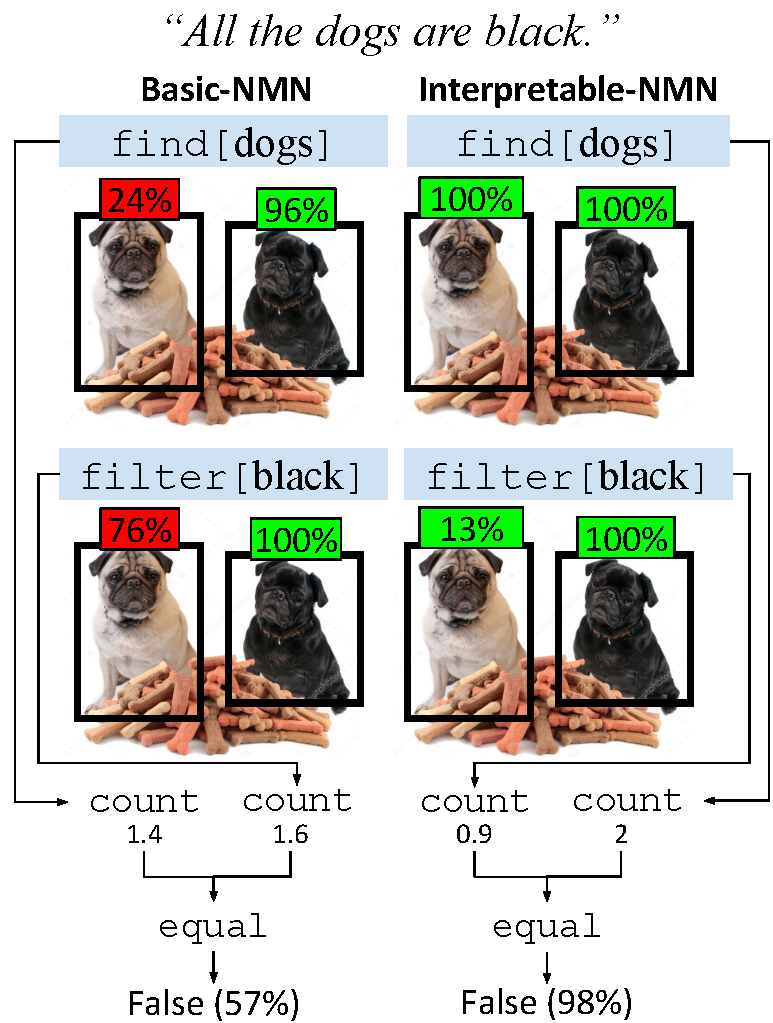
\includegraphics[width=62mm]{03-intro.pdf}
    \caption{An example for a visual reasoning problem where both the Basic and Interpretable NMNs produce the correct answer.
    The Basic NMN, however, fails to give meaningful intermediate outputs for the \texttt{find} and \texttt{filter} modules, whereas our improved interpretable-NMN assigns correct probabilities in all cases. Boxes are green if probabilities are as expected, red otherwise.}
    \label{fig:03-intro}
\end{figure}



\begin{figure}[tbh]
\centering
    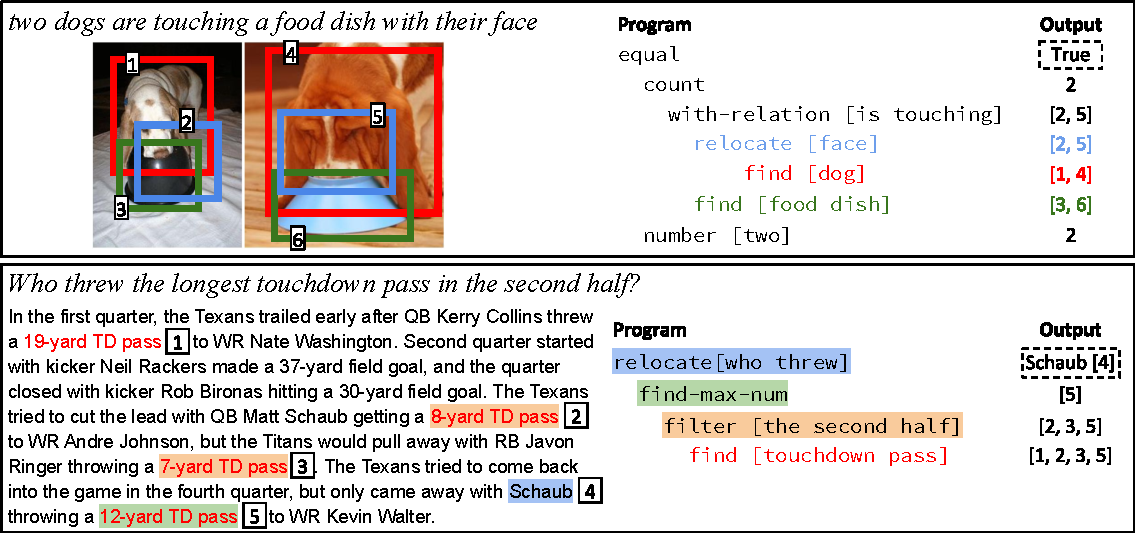
\includegraphics[width=0.9\textwidth]{03-combined.pdf}
    \caption{An example for a mapping of an utterance to a gold program and a perfect execution in a reasoning problem from \nlvr{} (top) and \drop{} (bottom).}
 \label{fig:03-nmn-example}
\end{figure}

% Neural module networks (NMNs;~\newcite{nmn-2016}) parse an input utterance into an executable program composed of learnable modules that are designed to perform atomic reasoning tasks and can be composed to perform complex reasoning against an unstructured context. NMNs are appealing since their output is interpretable; they provide a structured parse of the utterance and also the intermediate outputs performed to reach the final answer.
In a NMN, since module parameters are typically learned from end-task supervision only, it is possible that the model will solve the task, but the modules will not perform the reasoning steps as intended. In Figure~\ref{fig:03-intro}, a \emph{basic NMN} predicts the correct answer \texttt{False}, but does not correctly locate one of the \emph{dogs} in the image. This is undesirable, since the motivation for NMNs in this case is interpretability.
While recent work~\cite{explainablenmn-hu-2018,jiang-nmn-2019}, and even ours in Chapter 2, has shown that one can obtain good performance when using NMNs, interpretability was mostly evaluated through qualitative analysis, rather than systematically evaluating the intermediate outputs of each module.

In this chapter we provide three primary contributions regarding interpretability in NMNs.
First, we propose the concept of \emph{module-wise interpretability} -- a systematic evaluation of individual module performance that judges whether they have learned their intended operations, and define metrics to quantify this for both textual and visual reasoning (\S\ref{ssec:measure}).
Second, we provide strategies for improving module-wise interpretability in NMNs (\S\ref{ssec:interpret}).
Specifically, (a) we demonstrate how module architecture affects interpretability,
(b) propose supervising module outputs with either a proxy task or heuristically generated data, and (c)
show that providing modules with uncontexualized token representations improves interpretability.

Empirically, we show on both \nlvr{}~\cite{nlvr2-suhr-2018} and \drop{} \cite{drop-2019} that training a NMN using end-goal supervision, even using \emph{gold programs}, does \emph{not} yield module-wise interpretability which can be improved using techniques proposed in this chapter.
% We show that the different strategies proposed in this work improve interpretability to a great extent, sometimes at the cost of modest degradation in end-task performance.
Figure~\ref{fig:03-intro} shows an example where our approach (\emph{Interpretable-NMN}) results in much more sensible module outputs as compared to the \emph{Basic-NMN}.


\subsection{Module-wise Interpretability}
\label{ssec:measure}
% Neural module networks facilitate interpretability of their predictions by describing the reasoning steps as the program modules, and providing the intermediate outputs of those steps during execution.
% For example, in Figure~\ref{fig:03-nmn-example}, all reasoning steps taken by both the Visual-NMN and Text-NMN are interpretable.
% However, because module parameters are learned from an end-task, there is no guarantee that the modules will learn to perform their intended reasoning.
% Work on NMNs thus far~\cite{explainablenmn-hu-2018,jiang-nmn-2019} has overlooked systematically evaluating interpretability, performing only qualitative/subjective analysis in this regard.

We introduce the concept of \textit{module-wise interpretability}, aimed at providing an evaluation of module performance in a trained NMN.
Module-wise interpretability evaluates whether each module has correctly learned its intended operation by judging the correctness of the \emph{intermediate} module outputs.
For example, in Figure~\ref{fig:03-nmn-example} (top), a model would be judged module-wise interpretable if the outputs of all the modules, \texttt{find}, \texttt{relocate}, and \texttt{with\_relation}, are correct.

% Along with an interpretability score for each module separately, we compute its micro-average, i.e., an overall interpretability score.
We provide gold programs when evaluating interpretability, to not conflate  interpretability with parser accuracy.

\paragraph{Measuring interpretability in Text-NMN}
As shown in Chapter 2, each module in Text-NMN produces a distribution over passage tokens which represents the selected spans in a soft manner.
In order to measure module-wise interpretability of Text-NMN, we
annotated the set of spans that should be output by each module in the gold program.
Ideally, modules like \texttt{find}, \texttt{filter}, etc., should predict high probability for tokens that appear in the gold spans and \textit{zero} probability for other tokens. For example, the relevant spans for each module are shown in Figure~\ref{fig:03-nmn-example} (bottom).

Concretely, we use a metric akin to cross-entropy loss to measure the deviation of the predicted module output $p_{\text{att}}$ from the gold spans  $S~=~[s_{1}, s_{2}, \ldots, s_{N}]$. Here each span $s_{i} = (t^{i}_{\text{start}}, t^{i}_{\text{end}})$ is annotated as the start and end tokens.
Interpretability for a module is measured by:
\begin{equation*}
    I = - \sum_{i=1}^{N}  \Bigg(\log \sum_{j = t^{i}_{\text{start}}}^{t^{i}_{\text{end}}} p_{\text{att}}^{j} \Bigg).
\end{equation*}
Here, lower cross-entropy corresponds to better interpretability of a module.

\paragraph{Measuring interpretability in Visual-NMN}
Similarly, we define a quantitative meausure of interpretability in Visual-NMN based on the overlap between gold and predicted bounding-boxes that should be output by each module in the program. For brevity, we omit the details and refer the reader to the accompanying paper.


\subsection{Improving Interpretability in NMNs}
\label{ssec:interpret}
Module-wise interpretability is affected by various factors; the choice of modules and their implementation, use of auxiliary supervision, and the use of contextual utterance embeddings. We discuss ways of improving interpretability of NMNs across these dimensions.

\subsubsection{Choice of modules}
\paragraph{Textual reasoning}
In the context of Text-NMN (on \drop{}), we study the effect of formal language (module choice) on interpretability.

First, we introduce an \texttt{extract-answer} module. This module bypasses all compositional reasoning and directly predicts an answer from the input contextualized representations. This has potential to improve performance, in cases where a question describes reasoning that cannot be captured by pre-defined modules, in which case the program can consist of the \texttt{extract-answer} module only.
However, introducing \texttt{extract-answer} adversely affects interpretability and learning of other modules, specifically in the absence of gold programs. First, \texttt{extract-answer} does not provide any interpretability. Second, whenever the parser predicts the \texttt{extract-answer} module, the parameters of the more interpretable modules are not trained. Moreover, the parameters of the encoder are trained to perform reasoning \emph{internally} in a non-interpretable manner. We study the interpretability vs. performance trade-off by training Text-NMN with and without \texttt{extract-answer}.

Second, consider the program \texttt{find-max-num(find[\textrm{touchdown}])} that aims to find the \textit{longest touchdown}.
\texttt{find-max-num} should sort spans by their value and return the maximal one; if we remove \texttt{find-max-num}, the program would reduce to \texttt{find[\textrm{touchdown}]},
and the \texttt{find} module would have to select the longest touchdown rather than all touchdowns, following the true denotation. More generally, omitting atomic reasoning modules pushes other modules to compensate and perform complex tasks that were not intended for them, hurting interpretability.
To study this, we train Text-NMN by removing sorting and comparison modules (e.g., \texttt{find-max-num} and \texttt{num-compare}), and evaluate how this affects module-wise interpretability.

\paragraph{Visual reasoning}
The \texttt{count} module always appears in \nlvr{} as one of the top-level modules (see Figures~\ref{fig:03-intro} and~\ref{fig:03-nmn-example}).
Its gold denotation (correct count value) would provide minimal feedback using which the \emph{descendant} modules in the program tree, such as \texttt{filter} and \texttt{find}, need to learn their intended behavior.

We study how the architectural design of such a high-level module affects the learning of other modules in the model. We try three different architectures for the \texttt{count} module with varying expressivity and see how it affects learning.
\textbf{Layer-count module} uses a linear projection from image attention, followed by a \textrm{softmax}. This architecture explicitly uses the visual features giving it greater expressivity compared to simpler methods. Since this implementation has access to the visual features of the bounding boxes, it can learn to perform certain tasks itself, without providing proper feedback to descendant modules.
\textbf{Sum-count module} on the other extreme ignores any visual features and simply computes the sum of bounding box probabilities. Being parameter-less, this architecture provides direct feedback to descendant modules. However, such a simple functional-form does not ignore low-probability boxes and bounding boxes that overlap.
\textbf{Graph-count module}~\cite{zhang-count-2018} is a middle ground between both approaches; it does not use visual features, but learns to ignore overlapping and low-confidence bounding boxes while introducing only a minimal number of parameters. Such an architecture should provide the required inductive bias for accurate learning of the task and also should propagate gradients in a manner that encourages correct learning of \emph{descendant} modules.

\subsubsection{Supervising module output}
In Chapter 2 we proposed heuristic methods to extract supervision for the \texttt{find-num} and \texttt{find-date} modules in \drop{}. On top of the end-to-end objective, we used an auxiliary objective that encourages these modules to output the ``gold" numbers and dates according to the heuristic supervision.
In this chapter we evaluate the effect of such supervision on the interpretability of both the supervised modules, as well as other modules that are trained jointly.

We similarly find auxiliary supervision for modules in Visual-NMN and pretrain modules using that. We show that such pre-training helps learning of modules. Details are ommited for brevity.

\subsubsection{Decontextualized word representations}
We show the effect of decontextualized question token representations only for Visual-NMN and omit details here. Please refer the accompanying paper.
% As seen in Chapter 2, the question argument to the modules is supplied as a soft attention vector over the question tokens. The token representations that the modules use are contextualized based on the complete question and hence contain global question information. In the context of Visual-NMN we study how such contextualization might affect learning by inputting to the modules de-contextualized representations of question argument.


\subsection{Experiments}
We demonstrate that training NMNs using end-task supervision only does not yield module-wise interpretability both for visual and textual reasoning. We then show that the methods proposed in this chapter are crucial for achieving interpretability and how different design choices affect it.

\paragraph{Experimental setup}
We use the Text-NMN introduced in Chapter 2 which is evaluated on the complete development set of DROP which does not contain any program supervision.  Module-wise interpretability is measured on $100$ manually-labeled questions from the development set, which are annotated with gold programs and the passage spans.
We perform similar evaluation for Visual-NMN that we skip from this document for brevity.

\paragraph{Interpretability evaluation}
As seen in Table~\ref{tab:03-drop-results}, when trained on \drop{} using question-program supervision, the model achieves an F$_1$ score of $62.7$ and an interpretability score of $6.8$.
When adding supervision for intermediate modules, we find that the module-wise interpretability score improves to $5.1$.
Similar to Visual-NMN, this shows that supervising intermediate modules in a program leads to better interpretability.

To analyze how choice of modules affects interpretability, we train without sorting and comparison modules  (\texttt{find-max-num}, \texttt{num-compare}, etc.). We find that while performance improves slightly, interpretability deteriorates significantly to $8.4$,
showing that modules that perform atomic reasoning are crucial for interpretability.
When trained without program supervision, removing \texttt{extract-answer} improves interpretability  ($10.4\rightarrow 9.0$) but at the cost of model performance ($63.4 \rightarrow 60.8$ F$_1$).
This shows that such a black-box module encourages performing compositional reasoning in a non-interpretable manner, but can improve performance by overcoming the limitations of pre-defined modules.

\begin{table}[tbh]
\small
\centering
\captionsetup{font=footnotesize}
\resizebox{1.0\textwidth}{!}{
\begin{tabular}{lccccccc}
\toprule
\multirow{2}[3]{*}{\textbf{Model}} &
\multirow{2}[3]{*}{\begin{tabular}{@{}c@{}}\textbf{Performance} \\ (F$_1$ Score)\end{tabular}} & \multirow{2}[3]{*}{\begin{tabular}{@{}c@{}}\textbf{Overall Interp.} \\ (cross-entropy$^{*}$ $\downarrow$) \end{tabular}} &
\multicolumn{5}{c}{Module-wise Interpretability$^{*}$ ($\downarrow$)} \\
\cmidrule(lr){4-8}
                            &    &                & find  & filter & relocate & min-max$^\dagger$ & find-arg$^\dagger$ \\
\midrule
Text-NMN w/o prog-sup     &      &      &       &      &      &      &       \\
\;\;\; w/  \texttt{extract-answer}         & 63.4 & 10.4 &  14.1 & 11.8 &  3.0 &  4.2 &  11.6 \\
\;\;\; w/o \texttt{extract-answer}         & 60.8 &  \textbf{9.0} &  11.3 & 10.9 &  \textbf{0.9} &  2.7 &  10.5  \\

\addlinespace

Text-NMN w/ prog-sup     &      &      &       &      &      &      &       \\
\;\; no auxiliary sup           & 62.7          &  6.8          &  7.7          &  \textbf{5.8} &  \textbf{0.9} &  \textbf{1.7} &  8.7 \\
\;\; w/o sorting \& comparison  & \textbf{63.8} &  8.4          &  9.8          &  7.4          &  1.0          &  2.2          &  10.7         \\
\;\; w/ module-output-sup       & \textbf{63.8} &  \textbf{5.1} &  \textbf{6.1} &  6.1          &  \textbf{0.9} &  2.0          &  \textbf{6.9} \\
\bottomrule
\end{tabular}
}
    \caption{Interpretability and performance scores for various NMNs on \drop{}.
    %Introducing a black-box module, \texttt{extract-answer}, results in better model performance, but significantly hurts interpretability.
    %Omitting modules that perform crucial atomic tasks, such as sorting and comparison, significantly hurt interpretability. Also, providing intermediate module output supervision improves interpretability.
    $^*$lower is better. $^\dagger$min-max is average interpretability of \texttt{find-min-num} and \texttt{find-max-num}; find-arg of \texttt{find-num} and \texttt{find-date}.}
    %\bb{We should probably give a name for each of the interpretability metric so that it will be clear that the numbers of the two tables are not of the same metric} \jb{Don't think we need to overview results} \jb{why no boldface in the module-wise for best result?}}
    \label{tab:03-drop-results}
\end{table}


\subsection{Conclusion}
In this chapter we introduce the concept of \emph{module-wise interpretability}; a systematic evaluation of interpretability in neural module networks (NMNs) for visual and textual reasoning. We show that na\"ive training of NMNs does not produce interpretable modules and propose several techniques to improve module-wise interpretability in NMNs.
We show how our approach leads to much higher  module-wise interpretability at a low cost to performance.
As future work we propose to study how such module-wise interpretability in NMNs affects their systematic generalization.


\biblio

\end{document}
